\documentclass[aspectratio=43, handout]{beamer}
%la opcion hangout es para complilar en modo imprimible
%\documentclass[hangout]{beamer}

\mode<presentation>
{
  \usetheme{Berkeley}
  \setbeamercovered{transparent}
  \setbeamertemplate{navigation symbols}{}
}

\usepackage[spanish]{babel}
\usepackage[utf8]{inputenc}
\usepackage{tikz}
\usepackage{textpos}
\usepackage{hyperref}
\usepackage{caption}
\captionsetup[figure]{labelformat=empty}

\setbeamertemplate{footline}[frame number]
%\usetikzlibrary{shapes,arrows}
\setbeamerfont{author}{size=\large}
\setbeamerfont{institute}{size=\normalsize\bfseries}
\setbeamerfont{title}{size=\Large\bfseries}
\setbeamerfont{subtitle}{size=\huge}

\definecolor{darkblue}{RGB}{51,51,179}
\setbeamercolor{bgcolor}{fg=white,bg=darkblue}

%\title[WSN]{Sistema de Monitoreo de Salud de Nodos WSN Alimentados a Energía Solar}
\subtitle{WSN}
\author[]{Esp. Ing. Juan V. Montilla C.}
\institute[CESE-FIUBA]{Carrera de Especialización en Sistemas Embebidos - Facultad de Ingeniería - Universidad de Buenos Aires}
\date{}

%\subtitle{Framework para aplicaciones de control de ambientes}
\titlegraphic{\includegraphics[width=5cm]{./imagenes/red.jpg}}


\subject{Sistema de Monitoreo de Salud de Nodos WSN Alimentados a Energía Solar. Carrera de Especialización en Sistemas Embebidos}
% This is only inserted into the PDF information catalog. Can be left
% out. 

\pgfdeclareimage[height=1.5cm]{university-logo}{./imagenes/logo-facu-inverso.png}
\logo{\pgfuseimage{university-logo}}


% If you wish to uncover everything in a step-wise fashion, uncomment
% the following command: 

\beamerdefaultoverlayspecification{<+->}
  
\begin{document}

%Captions sin el texto "Figure"
\setbeamertemplate{caption}{\raggedright\insertcaption\par}

%la magia del begingroup es para que titlepage quede centrada, sin eso queda
%corrida en el ancho del sidebar
%\begingroup
%\makeatletter
%\setlength{\hoffset}{-.5\beamer@sidebarwidth}
%\makeatother
%\begin{frame}[plain,noframenumbering]
%  \titlepage
%\end{frame}
%
%\endgroup


%-------------------------------------------------%
%-------------------------------------------------%
% PORTADA
%-------------------------------------------------%
%-------------------------------------------------%

\begingroup
\makeatletter
\setlength{\hoffset}{-.5\beamer@sidebarwidth}
\makeatother
\begin{frame}[plain,noframenumbering]
\begin{center}
%\vspace{5px}
\hfill
    \begin{beamercolorbox}[center,dp=3ex,ht=10.25ex, wd=1\linewidth]{bgcolor}
        \Large\textbf{Sistema de Monitoreo de Salud de Nodos WSN Alimentados a Energía Solar}\\
       % \huge\textbf{802.15.4 LR-WPAN}
    \end{beamercolorbox}
\hfill\hfill
\\
\vspace{5px}
\textbf{Trabajo Final}\\
\textbf{Carrera de Especialización en Sistemas Embebidos}\\
\textbf{Facultad de Ingeniería - Universidad de Buenos Aires}\\

\vspace{10px}

\begin{figure}[H]
	\includegraphics[width=.3\textwidth]{./imagenes/red.jpg}
\end{figure}	 
\vspace{10px}
\texttt{Esp. Ing. Juan V. Montilla C.}\\
 	  	
\vspace{5px}
\tiny Agosto 2016 

\end{center}
\end{frame}
\endgroup

%-------------------------------------------------%
%-------------------------------------------------%

\begin{frame}{\textbf{\LARGE{Organización de la presentación}}}
\fontsize{13pt}{13}\selectfont
  \tableofcontents
  % You might wish to add the option [pausesections]
\end{frame}
%
%

%-------------------------------------------------%
%-------------------------------------------------%
\section{Introducción General}
%-------------------------------------------------%
%-------------------------------------------------%

%-------------------------------------------------%
\subsection[Motivación]{Motivación}
%-------------------------------------------------%

\begin{frame}{\textbf{\LARGE{Motivación}}}
\fontsize{16pt}{16}\selectfont
	\begin{itemize}
		\item Dispositivos con fuente de\\alimentación autónoma.
		\vspace{10px}
		\item Se presenta un problema de autonomía/vida útil.
		\vspace{10px}
		\item Necesidad de detectarlo.
		\vspace{10px}
		\item ¿Soluciones?
	\end{itemize}
%Es util y anda bien
%Servicio a la bateria, mantenimiento	
\end{frame}

\begin{frame}{\textbf{\LARGE{Soluciones}}}
\fontsize{15pt}{15}\selectfont
\begin{minipage}[c]{1.0\linewidth}
	\begin{minipage}[c]{0.55\linewidth}
		\begin{itemize}
			\item Módulo fotovoltaico.
					\vspace{10px}
			\item Control de carga.
					\vspace{10px}
			\item Optimizar la vida útil de la batería.
					\vspace{10px}
			\item Extremadamente bajo consumo de potencia.
		\end{itemize}
		\end{minipage}
	\begin{minipage}[c]{0.4\linewidth}
		\begin{itemize}
			\item IEEE 802.15.4
		\end{itemize}		
		\begin{figure}[H]
			{\includegraphics[width=0.8\textwidth]{./imagenes/arquitectura}}
		\end{figure}	
	\end{minipage}
\end{minipage}
\end{frame}
%-------------------------------------------------%
\subsection[WSN]{¿Qué es WSN?}
%-------------------------------------------------%
\begin{frame}{\textbf{\LARGE{¿Qué es WSN?}}}
\fontsize{14pt}{14}\selectfont
\noindent Wireless Sensor Networks:\\
\textbf{Redes de Sensores Inalámbricos}.
\begin{minipage}[c]{1.0\linewidth}
	\begin{minipage}[c]{0.4\linewidth}
		\begin{figure}[H]			
		\includegraphics[width=1.2\textwidth]{./imagenes/WSN.jpg}
		\end{figure}	  	  	
	\end{minipage}
	\begin{minipage}[c]{0.58\linewidth}
			\vspace{20px}
		\begin{itemize}
			\item Medición inteligente.
			\vspace{5px}
			\item Domótica y seguridad.
			\vspace{5px}
			\item Juguetes interactivos.
			\vspace{5px}
			\item Electrónica de consumo.
			\vspace{5px}
			\item Cuidado de la salud.
			\vspace{5px}
			\item Agricultura.
			\vspace{5px}
			\item Comunicación Militar.
			\vspace{5px}
		\end{itemize}
\end{minipage}
\end{minipage}
\end{frame}

\begin{frame}{\textbf{\LARGE{¿Qué es WSN?}}}{\LARGE{Interfaz de usuario a través de un sumidero}}
\fontsize{15pt}{15}\selectfont
		%\noindent Interfaz de usuario a través de un sumidero
		\begin{figure}[H]			
		\includegraphics[width=0.55\textwidth]{./imagenes/RedDistribuida.png}
		\end{figure}	  	  	
\end{frame}
%-------------------------------------------------%
\subsection[Energía]{Implicaciones de Energía}
%-------------------------------------------------%
\begin{frame}{\textbf{\LARGE{Implicaciones de energía}}} 
\fontsize{15pt}{15}\selectfont
\begin{minipage}[c]{1.0\linewidth}
	\begin{minipage}[c]{0.55\linewidth}
		\begin{itemize}
			\item El modulo fotovoltaico y pocos componentes.
					\vspace{10px}
			\item Generador Eléctrico Solar Autónomo (GESA).
					\vspace{10px}
			\item Acceso reducido\\a red eléctrica.
					\vspace{10px}
		\end{itemize}

\end{minipage}
	\begin{minipage}[c]{0.40\linewidth}
		\begin{figure}[H]			
		\includegraphics[width=1.2\textwidth]{./imagenes/ks10t.jpg}
		\end{figure}	  	  	
	\end{minipage}
\end{minipage}
\end{frame}
%-------------------------------------------------%
%-------------------------------------------------%
\section{Introducción Específica}
%-------------------------------------------------%
%-------------------------------------------------%
%-------------------------------------------------%
%\subsection[Objetivos]{Descripción del trabajo}
%%-------------------------------------------------%
%\begin{frame}{\textbf{\LARGE{Objetivos}}}
%% El primer minipage es un marco para las otras dos, que parten la pantalla en dos horizontalmente.
%% Con 0.6\linewidth le indicás que porcentaje del ancho de la página debe tener la minipage
%\noindent Los objetivos del trabajo son los siguientes:
%\begin{itemize}
%%	\item Full-function device (FFD):\\ Capaz de ser PAN coordinator o coordinator. 
%%	\vspace{10px}
%
%	\item Desarrollar un software de supervisión de nodos Mote LSE con extensión de panel solar.
%	\item Implementar el sistema en n nodos desplegados en una red inalámbrica de área personal.
%	\item Gestionar el modo de operación del nodo en función de la tensión que entrega el circuito cargador y la proyección de la batería restante.
%	\item Supervisar la temperatura del entorno del nodo.
%	\item Reportar a un nodo central el estado de salud del nodo.
%	\item Fijar y leer en forma remota las alarmas/parámetros de configuración.
%	 \end{itemize}	
%\end{frame}

%-------------------------------------------------%
\subsection[Herramientas]{Herramientas}
%-------------------------------------------------%
\begin{frame}{\textbf{\LARGE{Herramientas - Nodo Mote LSE}}}

\begin{minipage}[c]{1.0\linewidth}
	\begin{minipage}[c]{0.6\linewidth}
\begin{itemize}
\item Microcontrolador NXP LPC1343.\\
   %\begin{itemize}
Procesador ARM Cortex-M3 de 32 bits @72MHz.\\
32kB de memoria Flash.\\
8kB de memoria SRAM.\\
   %\end{itemize}
\item Transceptor TI-2520\\+ Extensor TI-2591.
\item Controlador de carga bq24080.
\item Batería de Li-ion de 3.7V y 900mAh.
\item Sensores de luz y temperatura.
\item Antena y balun en microstrip.
\end{itemize}
	\end{minipage}
	\begin{minipage}[c]{0.35\linewidth}
		\begin{figure}[H]
			\vspace{35px}
			\includegraphics[width=0.8\textwidth]{./imagenes/mote(1).jpg}
		\end{figure}	  	  	
	\end{minipage}
\end{minipage}
\end{frame}

%--------------------------------------------------------------------%
\subsection[Plan]{Planificación}
%--------------------------------------------------------------------%
\begin{frame}[t]{\textbf{\LARGE{Planificación - AON}}}
		\begin{figure}[H]
			{\includegraphics[width=1\textwidth]{./imagenes/Aon.PNG}}
		\end{figure}	 
\end{frame}

%-------------------------------------------------%
%-------------------------------------------------%
\section{Diseño e Implementación}
%-------------------------------------------------%
%-------------------------------------------------%
%-------------------------------------------------%
\subsection[Hardware]{Hardware}
%-------------------------------------------------%
\begin{frame}{\textbf{\LARGE{Hardware - El Panel Solar}}}
\begin{center}
			\begin{figure}[H]
			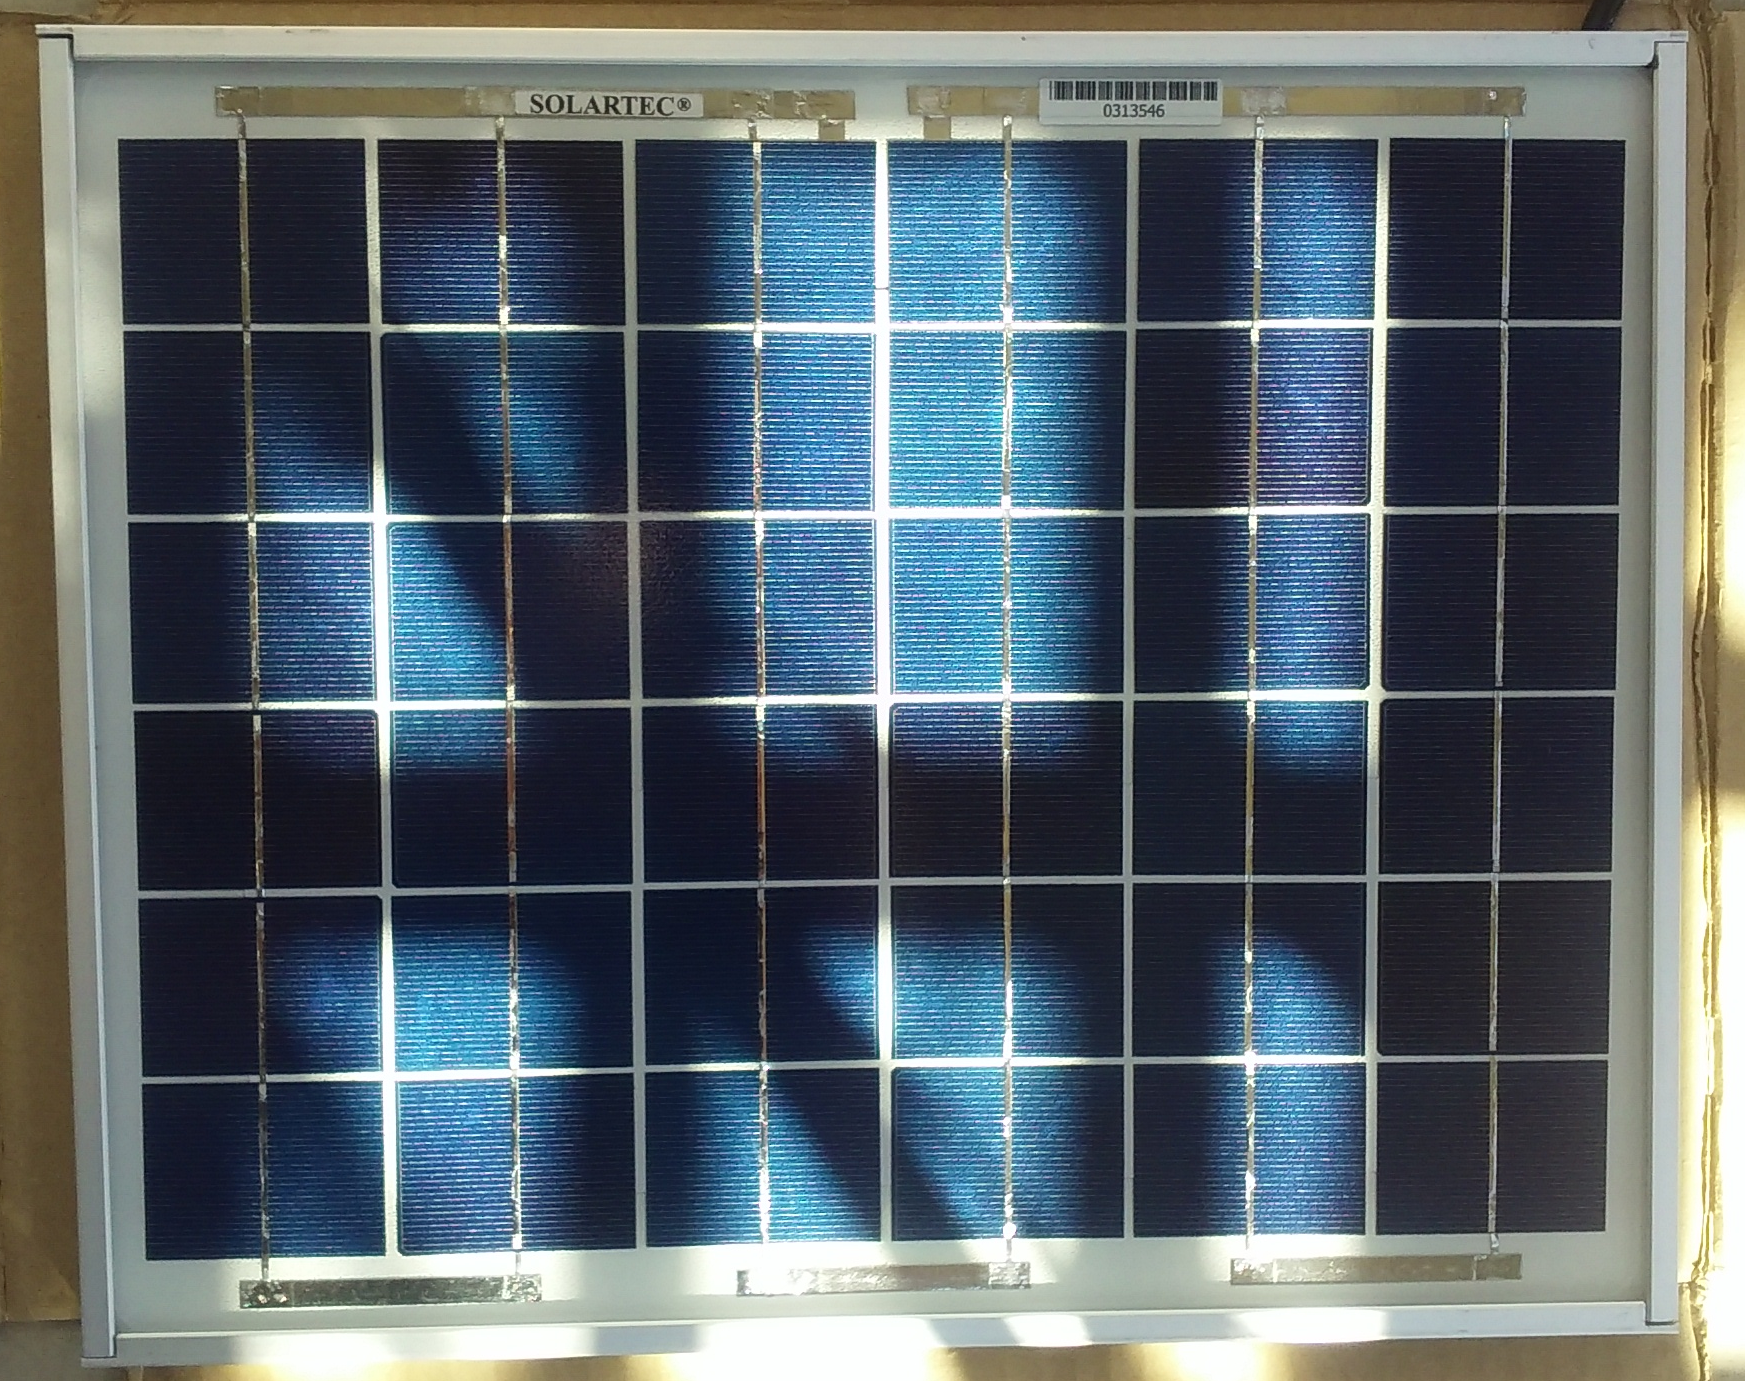
\includegraphics[width=0.5\textwidth]{./imagenes/panel.png}
			%\caption{Mote LSE}
		\end{figure}	
	\vspace{10px}	
	\begin{tabular}{@{} l *2c @{}}    %\toprule
		\hline
		\emph{\textbf{Características}} & \emph{\textbf{Valor}} & \emph{\textbf{Unidad}}\\
		%\midrule
		\hline
		Potencia nominal	& 10 	& Wp	\\	
		Tensión a PN		& 17.4	& V\\
		Corriente a PN	& 0.58		& A\\
		Dimensiones		& 301x352x22 	& mm\\
		Peso				& 0.58		& Kg	\\
		%\bottomrule
		\hline
	\end{tabular}
\end{center}
\end{frame}


\begin{frame}{\textbf{\LARGE{Hardware - Diagrama de Conexión}}}
		\begin{figure}[H]
			\includegraphics[width=1\textwidth]{./imagenes/conex.png}
			%\caption{Mote LSE}
		\end{figure}	
\end{frame}
%-------------------------------------------------%
\subsection[Arquitectura]{Arquitectura del Firmware}
%-------------------------------------------------%
\begin{frame}{\textbf{\LARGE{Arquitectura del Firmware}}}
\fontsize{14pt}{14}\selectfont
\begin{minipage}[c]{1.0\linewidth}
	\begin{minipage}[c]{0.4\linewidth}
		\begin{itemize}
			%\vspace{20px}
			\item APPS (Applications)
			\begin{itemize}
			\item cc2520Task
			\item monitoreoWsn
			\vspace{10px}
			\end{itemize}
			\item HAL (Hardware Abstraction Layer)
			\begin{itemize}
			\item Board Drivers
			\item 802.15.4
			\vspace{10px}
			\end{itemize}						
			\item Hardware
			\begin{itemize}
			\item Biblioteca de Cortex ARM: CMSISv2p00 LPC13xx
			%\vspace{10px}
			\end{itemize}
		\end{itemize}	
	  \end{minipage}
	  \begin{minipage}[c]{0.4\linewidth}
		\begin{figure}[H]
			{\includegraphics[width=1.5\textwidth]{./imagenes/arqcolor.PNG}}
		\end{figure}	  	  	
	  \end{minipage}
\end{minipage}

\end{frame}

%-------------------------------------------------%
\subsection[Firmware]{Firmware}
%-------------------------------------------------%

\begin{frame}{\textbf{\LARGE{Descripción Funcional}}}
\begin{figure}
	\centering
    \includegraphics[width=1\textwidth]{./imagenes/data.jpg}
    	\caption{Formato de la trama de Datos IEEE 802.15.4}
\end{figure}
\end{frame}

\begin{frame}{\textbf{\LARGE{Descripción Funcional}}}
\fontsize{15pt}{15}\selectfont
	\centering
	\noindent Estructura del payload (Disp$\rightarrow$Coord)
	\vspace{15px}
\begin{table}[ht]
	\centering
	\fontsize{8pt}{8}\selectfont

	\begin{tabular}{@{} l *6c @{}}    %\toprule
	\hline
		\emph{\textbf{Byte}} & \emph{\textbf{0}} & \emph{\textbf{1}} & \emph{\textbf{2}} & \emph{\textbf{3-4}} & \emph{\textbf{5}} & \emph{\textbf{6-127}}\\
		\hline
		Significado & Edo. de & Edo. de & Temp. & Voltaje & Ciclos & Datos\\
		 & Alarma & Operación & Amb. & Bat. & de Carga & \\
		\hline
	\end{tabular}
	\label{tab:dispcoor}
\end{table}
		\vspace{20px}
	\noindent Estructura del payload (Coord$\rightarrow$Disp)
\begin{table}[ht]
	\centering
	\fontsize{8pt}{8}\selectfont
		\vspace{15px}
	\begin{tabular}{@{} l *6c @{}}    %\toprule	
	\hline
		\emph{\textbf{Byte}} & \emph{\textbf{0}} & \emph{\textbf{1}} & \emph{\textbf{2}} & \emph{\textbf{3}} & \emph{\textbf{4}} & \emph{\textbf{5-127}}\\
		\hline
		Significado & Set & Ciclo & Límite & Límite & Límite & Datos\\
		 & Alarma & de Trabajo & Voltaje & Temp. Alta & Temp. Baja & \\
		\hline
	\end{tabular}
	\label{tab:coordisp}
\end{table}
\end{frame}

\begin{frame}{\textbf{\LARGE{Descripción Funcional}}}
	\fontsize{15pt}{15}\selectfont
		\centering
	\noindent Byte de Estado de Operación
\begin{table}[ht]
	\centering
	\fontsize{13pt}{13}\selectfont
	\begin{tabular}{@{} l *1c @{}}    %\toprule
	\hline
		\emph{\textbf{Valor}} & \emph{\textbf{Descripción}}\\
		\hline
		00000000 &  Modo Batería\\
		11111111 &  Modo Panel\\
		Otros & Reservado\\
		\hline
	\end{tabular}
	\label{tab:edoope}
\end{table}

\noindent Byte de Estado de Alarma
%\fontsize{13pt}{13}\selectfont
\begin{table}[ht]
	\centering
	\fontsize{13pt}{13}\selectfont
	\begin{tabular}{@{} l *1c @{}}    %\toprule
	\hline
		\emph{\textbf{Valor}} & \emph{\textbf{Descripción}}\\
		\hline
		00000000 & TempAmbaja\\	
		00000001 & TempAmbalta\\
		00000010 & ProyBatrest\\
		00000011 & TensionBat\\
		Otros & Reservado\\
		\hline
	\end{tabular}
\end{table}
\end{frame}

\begin{frame}{\textbf{\LARGE{Descripción Funcional}}}
\fontsize{15pt}{15}\selectfont
	\centering
\noindent Control de carga de la batería
\vspace{14px}
\begin{table}[ht]
	\centering
	\noindent Pines de estado del \textit{bq2480}
	\vspace{10px}
	\begin{tabular}{@{} l *3c @{}}    %\toprule
		\hline		
		\emph{\textbf{Estado}} & \emph{\textbf{STAT1}} & \emph{\textbf{STAT2}}\\
		\hline
		Precarga en progreso &  ON & ON \\	
		%Carga rápida en progreso	&  ON & OFF \\
		Carga completa &  OFF & ON \\
		Modo sleep &  OFF & OFF \\
		\hline
	\end{tabular}
	\label{tab:STAT}
\end{table}
\end{frame}

\begin{frame}{\textbf{\LARGE{Topología de la Red}}}
		\begin{figure}[H]
			{\includegraphics[width=.9\textwidth]{./imagenes/topologia.jpg}}
		\end{figure}	  	  	
\end{frame}

%-------------------------------------------------%
%-------------------------------------------------%
\section{Ensayos}
%-------------------------------------------------%
%-------------------------------------------------%
\begin{frame}{\textbf{\LARGE{Ensayos}}}
\begin{center}
		\begin{figure}[H]
			{\includegraphics[width=1\textwidth]{./imagenes/cargas.png}}
		\end{figure}	
		\vspace{5px} 
		Voltaje y Estados del Circuito Controlador de Carga\\
		vs Tiempo en estado de recarga
\end{center}	  	
\end{frame}

\begin{frame}{\textbf{\LARGE{Ensayos}}}
\begin{center}
		\begin{figure}[H]
			{\includegraphics[width=0.9\textwidth]{./imagenes/descargas.PNG}}
		\end{figure}	 
		\vspace{10px} 
		Voltaje y Estados del Circuito Controlador de Carga\\
		vs Tiempo en modo batería
\end{center}	 	  	
\end{frame}

\begin{frame}{\textbf{\LARGE{Demostración}}}
\begin{center}
		\begin{figure}[H]
			{\includegraphics[width=.9\textwidth]{./imagenes/debu.jpg}}
		\end{figure}	  
\end{center}	 	  	
\end{frame}

%-------------------------------------------------%
%-------------------------------------------------%
\section{Trabajos Futuros}
%-------------------------------------------------%
%-------------------------------------------------%
\begin{frame}{\textbf{\LARGE{Trabajos Futuros}}}
\fontsize{15pt}{15}\selectfont
	\begin{itemize}
			\item Implementación en otras plataformas (funcionalidades vs consumos).
			\begin{itemize}
			\fontsize{14pt}{14}\selectfont
			\item Temperatura de la batería.
			\item Corriente de carga de la batería.
			\item Consumo de corriente del circuito.
			\end{itemize}
			\vspace{10px}
			\item Implementación con otros algoritmos.
			\vspace{10px}
			\item Soporte a las plataformas disponibles del Proyecto CIAA.
	\end{itemize}	  	
\end{frame}

%%-------------------------------------------------%
%%-------------------------------------------------%
%\section{Referencias}
%%-------------------------------------------------%
%%-------------------------------------------------%
%
%\begin{frame}[c]{Referencias}
%
%%\Large{Referencias}
%\vspace{20px}
%\begin{itemize}
%	\item<.-> \href{http://ecee.colorado.edu/~liue/teaching/comm_standards/2015S_zigbee/802.15.4-2011.pdf}{Estándar IEEE 802.15.4:2011}
%	\vspace{5px}	
%	\item<.-> \href{http://www.ieee802.org/15/pub/TG4.html}{IEEE 802.15 - Task Group 4 - Home Page}
%	\vspace{5px}
%	\item<.-> \href{	https://standards.ieee.org/about/get/802/802.15.html}{IEEE Get Program}
%	\vspace{5px}
%	\item<.-> \href{http://www.nxp.com/documents/data_sheet/LPC1311_13_42_43.pdf}{LPC1343 - Datasheet}
%	\vspace{5px}
%	\item<.-> \href{http://www.nxp.com/documents/user_manual/UM10375.pdf}{LPC1343 - User Manual}
%	\vspace{5px}
%	\item<.-> \href{http://www.ti.com/product/CC2520/technicaldocuments}{Texas Instrument CC2520 -  Technical Documents}
%	\vspace{5px}
%	\item<.-> \href{http://www.ti.com/lit/an/swru120b/swru120b.pdf}{Texas Instrument Design Note - 2.4 GHz Inverted F Antenna}
%\end{itemize}
%\end{frame}

%\section*{cartón de gracias}

\begingroup
\makeatletter
\setlength{\hoffset}{-.5\beamer@sidebarwidth}
\makeatother
\begin{frame}[plain,noframenumbering]
\begin{center}
%\vspace{5px}
\hfill
    \begin{beamercolorbox}[center,dp=3ex,ht=10.25ex, wd=1\linewidth]{bgcolor}
        \Large\textbf{Sistema de Monitoreo de Salud de Nodos WSN Alimentados a Energía Solar}\\
    \end{beamercolorbox}
\hfill\hfill
\\
\vspace{5px}
%\textbf{Trabajo Final}\\
%\textbf{Carrera de Especialización en Sistemas Embebidos}\\
%\textbf{Facultad de Ingeniería - Universidad de Buenos Aires}\\
\vspace{10px}
\texttt{\LARGE{¿Preguntas?}}\\

\vspace{10px}

\begin{figure}[H]
	\includegraphics[width=.3\textwidth]{./imagenes/red.jpg}
\end{figure}	
\vspace{10px}
\texttt{Esp. Ing. Juan V. Montilla C.}\\

\vspace{5px}
\tiny Agosto 2016 
 	  	
\end{center}
\end{frame}
\endgroup

\end{document}
